\documentclass[UTF8,fontset=ubuntu]{ctexart}
\usepackage{graphicx}
\usepackage{float}
\begin{document}
\begin{verbatim}
一、Demo(示例)01 - itemize list
\documentclass{article}
\begin{document}
	\begin{itemize}
		\item Each list item is marked with a label. The labels in this itemized list are bullets.
		\item \LaTeX\ permits at least four levels of nested lists, which is more than enough.
		\item Blank lines before an item have no effect.
	\end{itemize}
\end{document}

内容讲解
1.\begin{itemize} ... \end{itemize}用于非序号列表

2.\item[num]为列表项内容, num用于指定编号内容



二、Demo(示例)02 - enumerate list
\documentclass{article}
\begin{document}
	\begin{enumerate}
		\item The item labels in an enumerated list are numerals or letters.
		\item A list should have at least two items.
	\end{enumerate}
\end{document}

内容讲解
1.\begin{enumerate} ... \end{enumerate}用于序号列表

2.\item为列表项内容



三、Demo(示例)03 - description list
\documentclass{article}
\begin{document}
	\begin{description}
		\item[gnat] A small animal, found in the North Woods, that causes no end of trouble.
		\item[gnu] A large animal, found in crossword puzzles, that causes no end of trouble.
		\item[armadillo] A medium-sized animal, named after a medium-sized Texas city.
	\end{description}
\end{document}

内容讲解
1.\begin{description} ... \end{description}用于描述性列表

2.\item为描述性列表项内容, []为列表项名称



四、Demo(示例)04 - list
documentclass{article}
\newcounter{bean}
\begin{document}
    Alice was beginning to get very tired of sitting by her sister on the
bank, and of having nothing to do: once or twice she had peeped into

    \begin{list}{B--\Roman{bean}}{\usecounter{bean}\setlength{\parindent}{1cm}}
        \item Each list item is marked with a label. The labels in this itemized list are bullets.

        this is second paragraph
        \item \LaTeX\ permits at least four levels of nested lists, which is more than enough.
        \item[train] Blank lines before an item have no effect.
    \end{list}

    Alice was beginning to get very tired of sitting by her sister on the
\end{document}

内容讲解
1.\begin{list}{label_fmt}{list_struct} ... \end{list}用于指定list环境;
	label_fmt为列表entry的默认label; 
	list_struct用于调整list的计数器和元素间隔. 
	label_fmt和list_struct格式参考4/5

2.\item[label]指定entry内容, label用于指定label, 该内容覆盖1中的默认label

3.\newcounter{counter}创建新计数器, 初始数字为0

4.label_fmt参数列表:
	\Roman{counter} - 使用大写罗马格式计数, 计数格式如下:
		arabic - 阿拉伯数字	
		roman - 小写罗马数字
		Roman - 大写罗马数字
		alph - 小写字母
		Alph - 大写字母
		
5.list_struct结构参数列表(参考下图):
\end{verbatim}
\begin{figure}[H]
\graphicspath{{./picture/}}
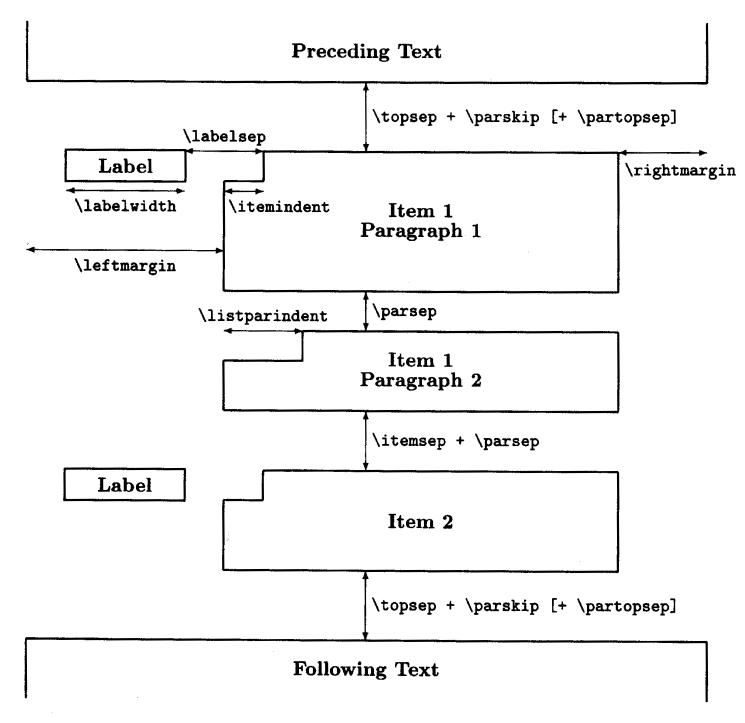
\includegraphics[scale=0.4]{list_layout}
\caption{引用自Leslie Lamport - A Document Preparation System\\
\centering Figure 6.3: The format of a list}
\end{figure}
\begin{verbatim}
	\usecounter{counter} - 特定用于list环境的第二个参数, 可在列表中使用指定计数器
	\topsep - 与partopsep、parskip组合, 称为外部文本与list的垂直距离(list上/下部分)
	\partopsep - 与topsep、parskip组合, 成为外部文本与list的垂直距离, 默认为0pt
	\labelsep - label与item首行的水平距离. label与item的距离为labelsep-itemindent
	\itemindent - item首行缩进
	\listparindent - item内, 除第一段的段落缩进
	\parsep - item内, 段落之间的垂直间距
	\itemsep - item之间, 指定的额外距离. 实际item之间的距离为itemsep+parsep
	\leftmargin - item实际内容(label右侧文本内容)左侧距离外部文本内容左侧的水平距离
	\rightmargin - item实际内容(label右侧文本内容)右侧距离外部文本内容右侧的水平距离
\end{verbatim}
\end{document}
